\documentclass[11pt]{article}
\usepackage{fullpage}
\usepackage{hyperref}
\usepackage{listings}
\usepackage{graphicx}
\graphicspath{ {figs/} }

%\usepackage{doublespace}
\begin{document}
\title{Weekly Report - Diving into the Ethminer Source Code}
\author{MSc Project \\
Runchao Han \\
}
\maketitle
%
% This section is used to list the key action items from the
% previous meeting. This information will help provide 
% continuity of information and decisions made in the
% previous meeting. 
% Use the \item construct to list each item.  Try to keep the
% descriptions for each down to one or two sentences
%

%TODO references
\section{Progress of the Last Week}

\begin{enumerate}
\item Imported \texttt{Ethminer} and \texttt{CCMiner} projects to IDEs (QtCrator, Codeblocks)
\item Learned about the Ethash implementation of \texttt{Ethminer} 
\item Learned about \texttt{GNU Make}, \texttt{CMake} and \texttt{CUDA}
\end{enumerate}

\section{Building C/C++ Projects by make/cmake}

(I have had no knowledge about the GCC toolchain before this, so I wrote this brief summary)

Most of blockchain projects are written by C++, especially the mining modules. To develop a big project, automatic building tools are applied throughout the development. \texttt{GCC}\footnote{https://gcc.gnu.org/} toolchain is the most widely used tools for C/C++ projects, which includes:

\begin{itemize}
\item GNU make: an automation tool for compilation and build
\item GNU Compiler Collection (GCC): a suite of compilers for several programming languages
\item GNU Binutils: a suite of tools including linker, assembler and other tools
\item GNU Bison: a parser generator, often used with the Flex lexical analyser
\item GNU m4: an m4 macro processor
\item GNU Debugger (GDB): a code debugging tool
\item GNU build system (autotools): Autoconf, Automake and Libtool
\end{itemize}

This section mainly talks about building related projects.

\subsection{Automatically Building Projects by make}

\texttt{GNU Make}\footnote{https://www.gnu.org/software/make} is the automatic building toool for C/C++ projects. By writing user-defined rules in the \texttt{Makefile} the \texttt{make} command will compile the project automatically following the rules.

\subsection{Cross-platform Building Tool cmake}

Besides \texttt{GNU Make}, a wide range of automatic building tools exist, like \texttt{Qmake} and \texttt{MS Nmake}. Moreover, cross-platform compiling is always an issue when building a project. 

\texttt{CMake} aims at designing a platform-independent makefile \texttt{CMakeList.txt} which can generate specific makefiles in specific environments so that the building process can be customised. For example, with the \texttt{CMakeList.txt}, the \texttt{Makefile} of \texttt{GNU Make}, the \texttt{Microsoft Visual Studio} project file can be generated. 

\subsection{Process of Building Ethminer}

\texttt{Ethminer} project is built upon \texttt{CMake}, so the process is:

\begin{enumerate}
\item \texttt{cd}: the project directory
\item \texttt{mkdir ./build}: generate a folder for the future generated \texttt{GNU Make} project
\item \texttt{./configure}: check dependencies
\item \texttt{cd buld \&\& cmake .. -DETHASHCUDA=ON}: to generate a \texttt{GNU Make} project from the \texttt{CMakeList.txt} with CUDA (CUDA is not included by default)
\item \texttt{make}: compile the whole project
\end{enumerate}

\section{Importing cmake/make Project Into IDEs}

IDEs like Codeblocks and QtCreator maintain their own project files instead of  \texttt{Makefile} or \texttt{CMakeList.txt}. Therefore, issues of importing projects exist.

\subsection{Importing CMake Project to IDEs}

To import the \texttt{Cmake} project, we can:

\begin{itemize}
\item Use inherited \texttt{cmake -g} command to generate the specific project file for the corresponding IDE. For example, \texttt{cmake .. -G"CodeBlocks - Unix Makefiles"} generates the \texttt{Codeblocks} project file with the existing \texttt{CMakeList.txt}
\item Some IDEs can import projects by \texttt{CMakeList.txt}, like \texttt{QtCreator}.
\end{itemize}

\subsection{Importing Make Project to IDEs}

As for \texttt{GNU Make} projects, no inherited project file generation methods exist. So if the chosen IDE does not support importing \texttt{Make} projects, we can only copy and paste.

Currently I'm not sure which IDE has better support for CMake/Make projects.

\section{Ethminer Source Code Explained}

\texttt{Ethminer}\footnote{https://github.com/ethereum-mining/ethminer} is a fairly huge project supporting mining in a mining pool, which implements the Ethash PoW algorithm.

\subsection{Ethminer Project Structure}

The project consists of the main program with libraries. All subdirectories are listed below:

\begin{itemize}
\item ethminer: The main miner program
\item libapicore: API for connecting to mining pools
\item libdevcore: Classes related to codings (e.g. RLP coding) and producing logs
\item libethash: Classes implementing common submodules for Ethash, like FNV Hash and SHA3, but the core algorithm is not in this directory
\item libethash-cl/cuda: The core implementation of Ethash by OpenCl/CUDA
\item libethcore: Classes from the Ethereum required by the mining process, like the main Miner class
\item libstratum: Stratum is the future mining protocol for cryptocurrencies. Currently it is optional to install and not adopted by any mainstream blockchains.
\end{itemize}

As for profiling the mining algorithm, we mainly care about \texttt{ethminer}, \texttt{libethash}, \texttt{libethash-cuda} and \texttt{libethcore} subdirectories.

\subsection{CUDA Mining Module Explained}

A brief class/invocation diagram is drawn in Fig.~\ref{fig:ethminer_ethash_classdiagram} showing the invocation order of the Ethash mining process.

\begin{figure}[h]
    \centering
    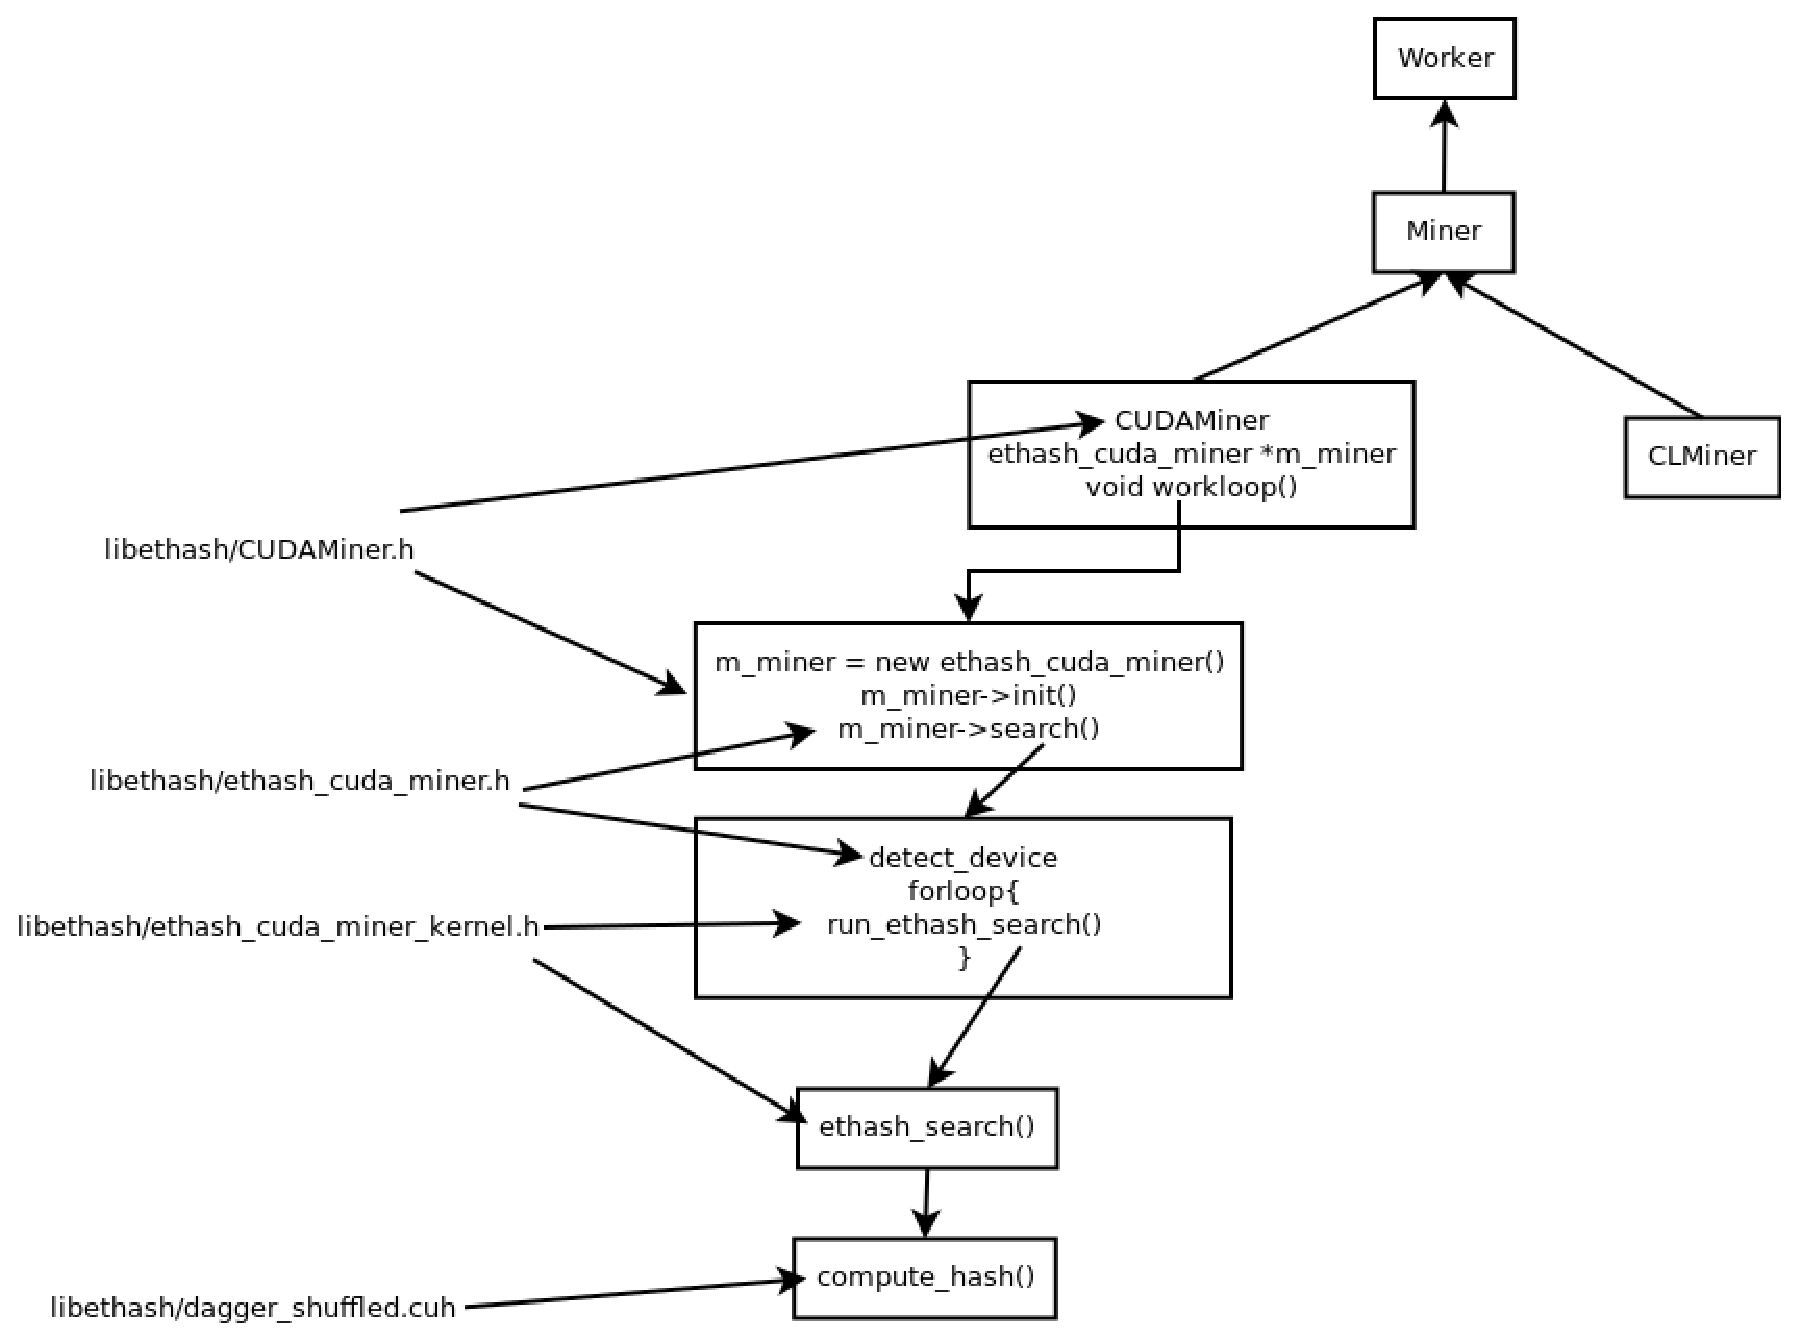
\includegraphics[width=0.8\textwidth]{ethminer_ethash_classdiagram.eps}
    \caption{An informal class diagram of Ethminer.}
    \label{fig:ethminer_ethash_classdiagram}
\end{figure}

Currently it is confirmed that $compute\_hash()$ in Fig.~\ref{fig:ethminer_ethash_classdiagram} is the $hashimoto()$ process in the Ethash Wiki\footnote{https://github.com/ethereum/wiki/wiki/Ethash}, which is parallelised by CUDA.

CUDAMiner class is the main mining program which controls the whole mining process, like kickoff(), pause() and GPU configurations. 

$libethash/ethash\_cuda\_miner\_kernel.h$ also contains the DAG generation and cache generation functionalities.

\section{Miscellaneous}

\begin{itemize}
\item I'm not sure which IDE I should use (QtCreator seems to have poor support for CMake projects.), which needs further research.
\end{itemize}
%
% This section is used to list the following week's plan
% Use the \item construct to list each item.  Try to keep the
% Descriptions for each down to one or two sentences
%
\section{Next Week's Plan}
\begin{enumerate}
\item Add timestamps to the Ethash implementation to make analysis
\item Import ccminer to IDE
\item Output stack graphs if I can
\end{enumerate}

No reference this week because the work in this week is about setting up the programming environment and reading the source code.

%\bibliographystyle{plain}
%\bibliography{references.bib}

\end{document}
